\section*{Results}

\begin{figure}
	\centering
	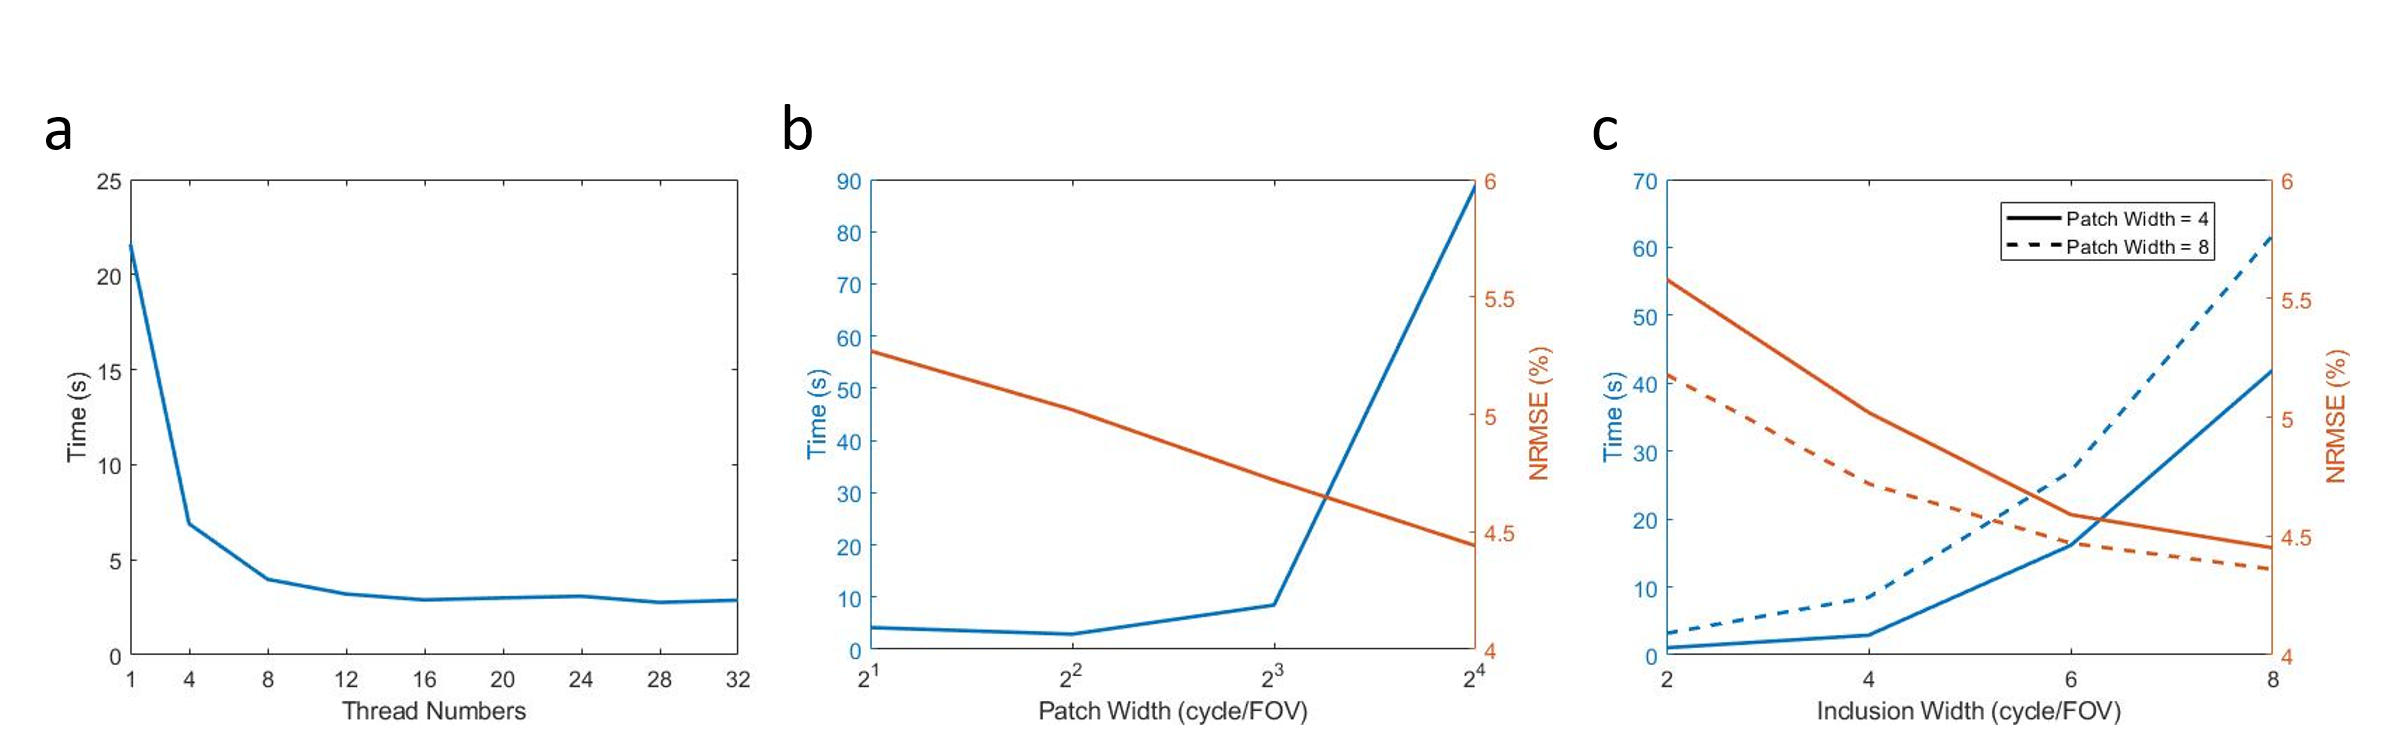
\includegraphics[width=\textwidth]{kspace_PTX_ComputationTime}
	\caption{Studies of different parallelization parameters, where patch width is the square root of the number of $\mathbf{W}$ columns solved for simultaneously and inclusion width is the assumed range of influence of each excitation k-space location. \textbf{(a)} Computation time vs. thread numbers. Patch width and inclusion with were kept at 4 cycle/FOV. \textbf{(b\&c)} Computation time (blue axis) and NRMSE (red axis) vs. patch widths (b) and inclusion widths (c). Thread number were kept at 16 of for both design. Inclusion width was constant at 4 in (b) and patch widths were constant at 4 (solid line) and 8 (dashed line).}
	\label{fig:ComputationTime}
\end{figure}
Figure \ref{fig:ComputationTime}a shows the mean computation time versus different thread numbers. The k-space design problem held the patch and inclusion width constant at 4. The mean computation time decreases with increasing thread numbers before 12 threads, and then plateaus due to overhead. The thread number was conservatively chosen to be 16 for the following studies to ensure timely solutions. 
Figure \ref{fig:ComputationTime}b shows the mean computation time and the NRMSE with different patch widths. The computation time increases and the NRMSE decreases as the patch width increases. This was because when patch width increases, there are more excitation trajectory points included in one instance problem, even with the same inclusion width. As a result, each instance problem becomes bigger and more time consuming, which cancels the advantageous fact that there are fewer instance problems in total, especially in cases with parallel computing. Furthermore, increasing the patch width is equivalently increasing the inclusion widths for the center target points within each patch, which makes the solutions more accurate. Here, we chose patch widths 4 and 8 (labeled $2^2$ and $2^3$) to balance time and accuracy for further evaluation.
Figure \ref{fig:ComputationTime}c shows the mean computation time and the NRMSE with different inclusion widths. The solid lines and dashed lines were obtained with patch width 4 and 8, respectively. Computation time increases and error decreases with increasing inclusion width. Particularly, increasing inclusion width is equivalent to utilizing more accurate $B_1^+$ information by truncating the $B_1^+$ map Fourier transforms to zero further out from DC. For both patch widths 4 and 8, 4 is the optimal inclusion width, which confirms the result in \ref{fig:ComputationTime}a , previously. Using an inclusion width of 4, the computation time and error are acceptable for both patch width numbers. Following these results,  we chose patch width 4 for the further designs.

\begin{figure}
	\centering
	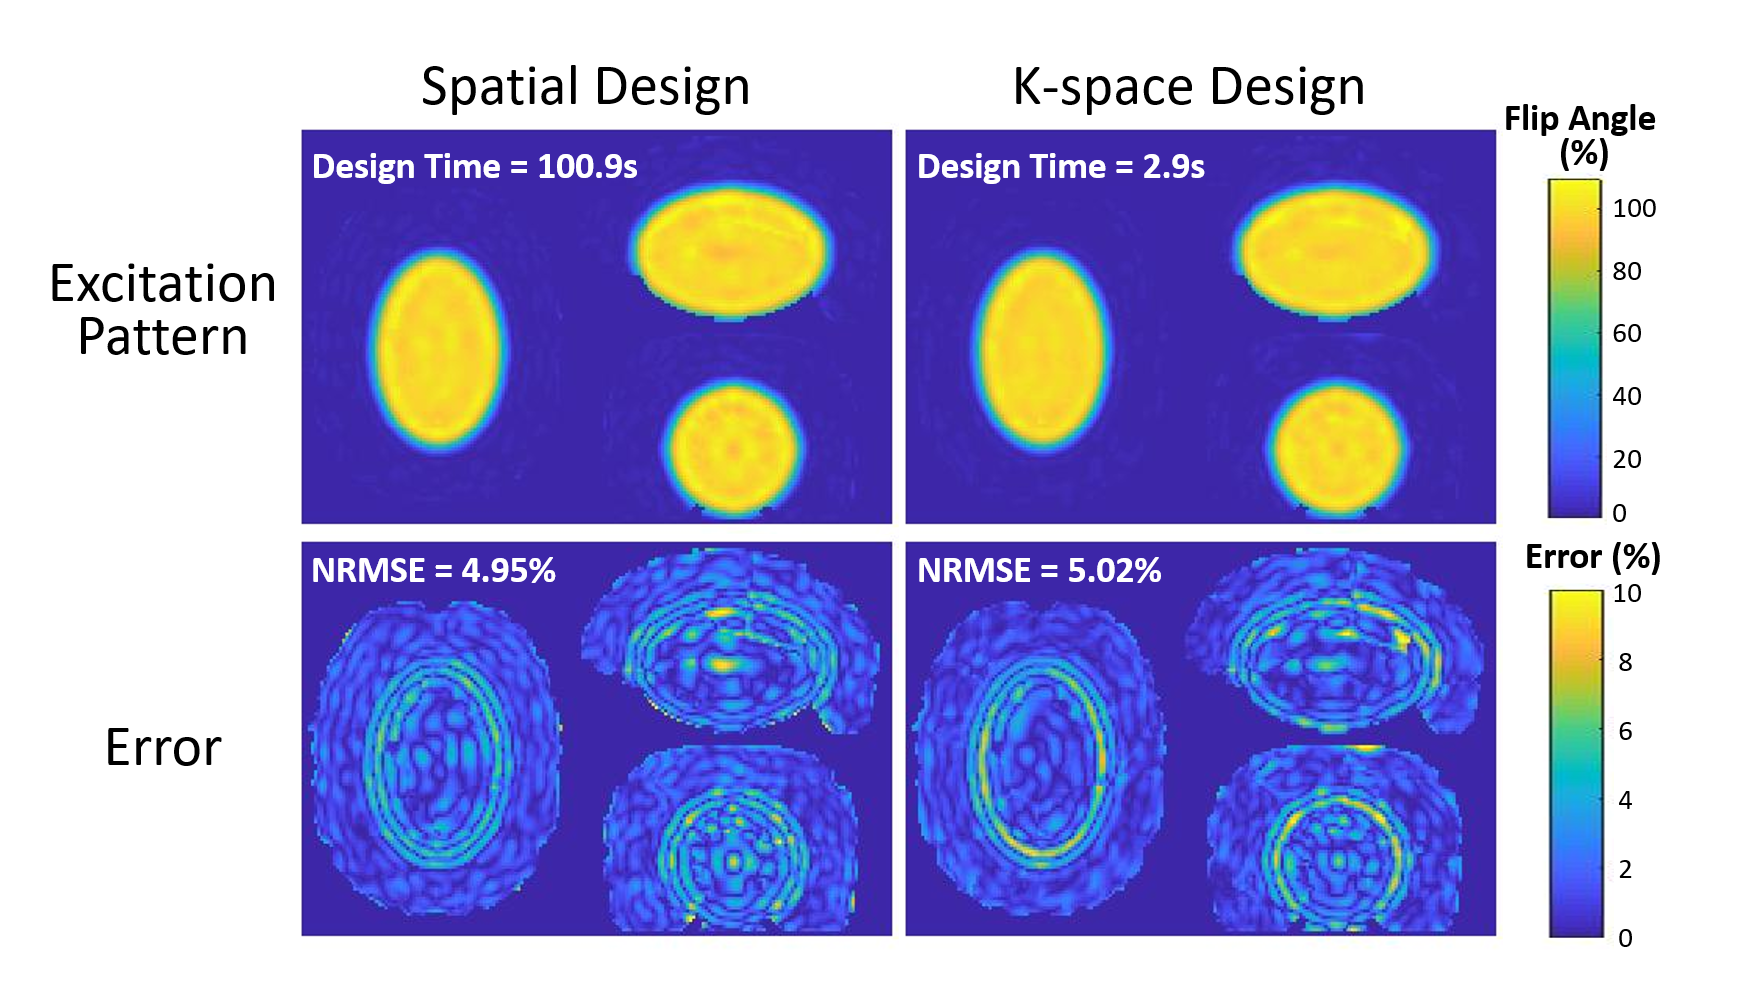
\includegraphics[width=\textwidth]{kspace_PTX_ErrorMap2}
	\caption{Normalized excitation patterns (top row) and error maps (bottom row) for k-space domain design (left column) and spatial domain design (right column), with NRMSE and design time indicated.}
	\label{fig:ErrorMap}
\end{figure}
The normalized excitation patterns and error maps are shown in Fig \ref{fig:ErrorMap} for both k-space domain design (left) and spatial domain design (right), where the k-space domain design was solved with 16 parallel computing threads, patch width 4, and inclusion width 4. 
Both designs were done with the 64$\times$64$\times$48 grid size (3mm iso-resolution), and the excitation patterns were evaluated against the target pattern with the 128$\times$128$\times$96 grid size (1.5mm iso-resolution).  grid size. 
The calculated NRMSE from the k-space domain design and the spatial domain design were 5.02\% and 4.94\%, respectively, which were practically equal. For both design methods, most of the errors appeared at the edges of the transition band, with other errors lower than 5\% of the target flip angle. This indicates uniform inner volume suppression while maintaining the outer volume intact, which can in turn decrease g-factor in highly accelerated imaging. In practice, error near the transition band can be mitigated by ensuring the region of interest (ROI) of the cortex falls completely in the stop-band and assuming zero signal within the pass-band during undersampled reconstruction. More significantly, the parallelized k-space domain design method drastically reduced the mean computation time from 100.9 seconds to 2.9 seconds compared to the spatial domain design, which was a 97\% decrease.

\begin{figure}
	\centering
	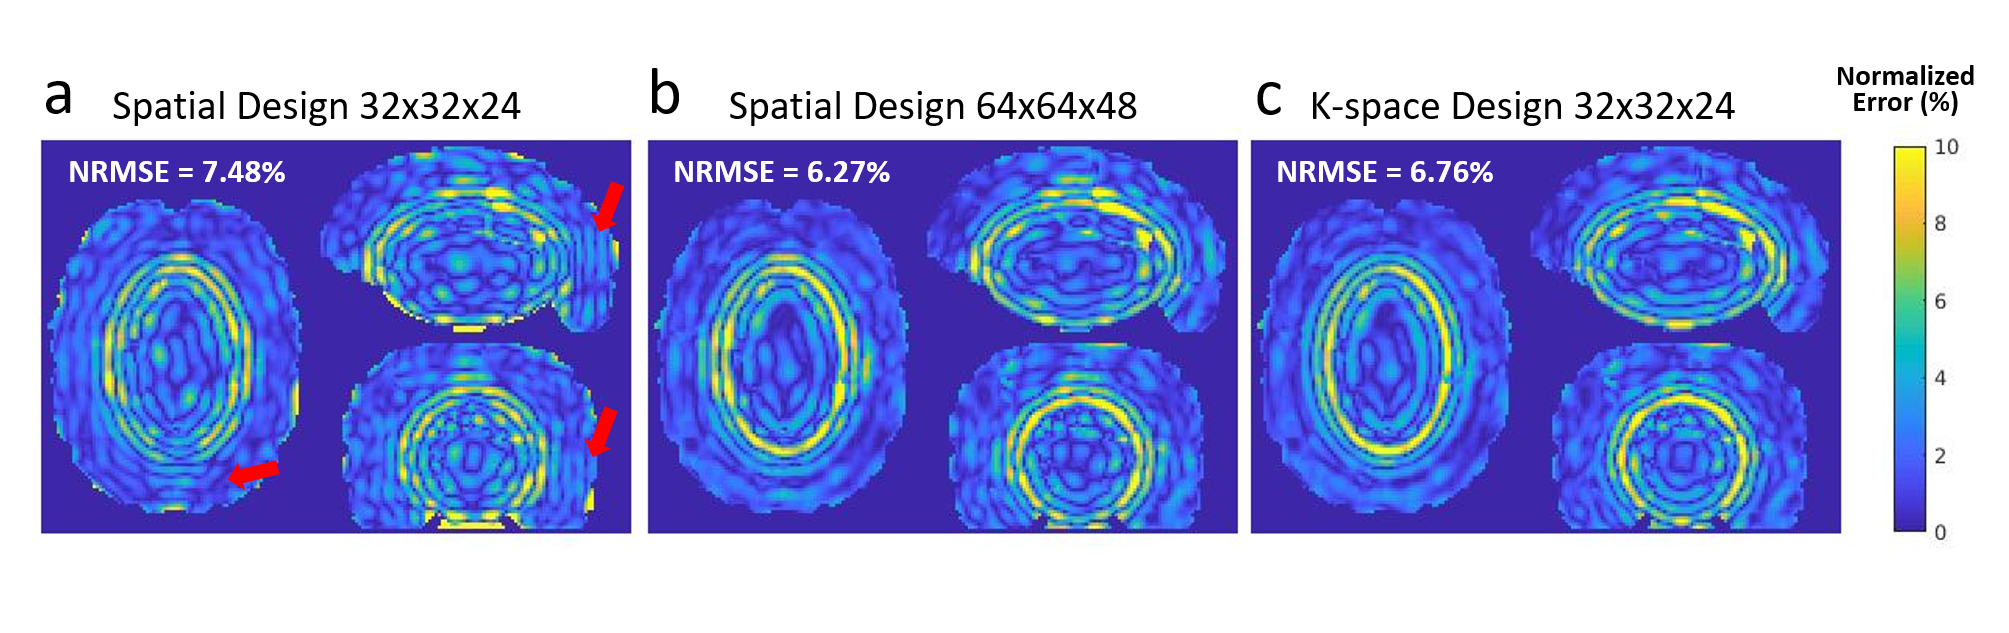
\includegraphics[width=\textwidth]{kspace_PTX_GibbsRinging}
	\caption{Normalized error maps and NRMSE for \textbf{(a)} spatial domain design and \textbf{(c)} k-space domain design with 6 mm iso-resolution, 32$\times$32$\times$24 design grid. Red arrows indicate the Gibbs ringing in low-resolution spatial domain design. \textbf{(b)} Normalized error map for spatial domain design with 3 mm iso-resolution, 64$\times$64$\times$48 design grid.}
	\label{fig:GibbsRing}
\end{figure}

Figure \ref{fig:GibbsRing}a\&c show the results of the  low-resolution designs using k-space domain method and the spatial domain method. The result of the high-resolution design of the spatial domain is also shown in Figure \ref{fig:GibbsRing}b. All three designed were done with a excitation trajectory that matches the 6 mm iso-resolution. The red arrows indicate the Gibbs ringing in the low-resolution spatial domain design, that can only be suppressed with high-resolution spatial domain design. However, the k-space domain design, although also low-resolution, is insensitive to this problem. Furthermore, the ripple pattern in the low resolution k-space design matches the high-resolution spatial design. Looking from a spatial domain point of view, the Gibbs ringing was caused by the lack of ability to observe the ringing with low-resolution. Looking from a k-space domain point of view, the Gibbs ringing was due to "wrap back" of the k-space FOV. When the spatial resolution is low the k-space FOV is small, and therefore the RF samples at one end of the trajectory can incorrectly "reach" and affect the k-space points at the other end of the k-space FOV in a circulation shift fashion. However, for the k-space domain design, even with low resolution, there is no k-space "wrap back" because the incorporated trajectory points are explicitly specified. Particularly, for the instance problems whose patches are at the edges of the k-space FOV, the excitation trajectory points at the other ends of the k-space FOV will not be incorporated into the design.    


\begin{figure}
	\centering
	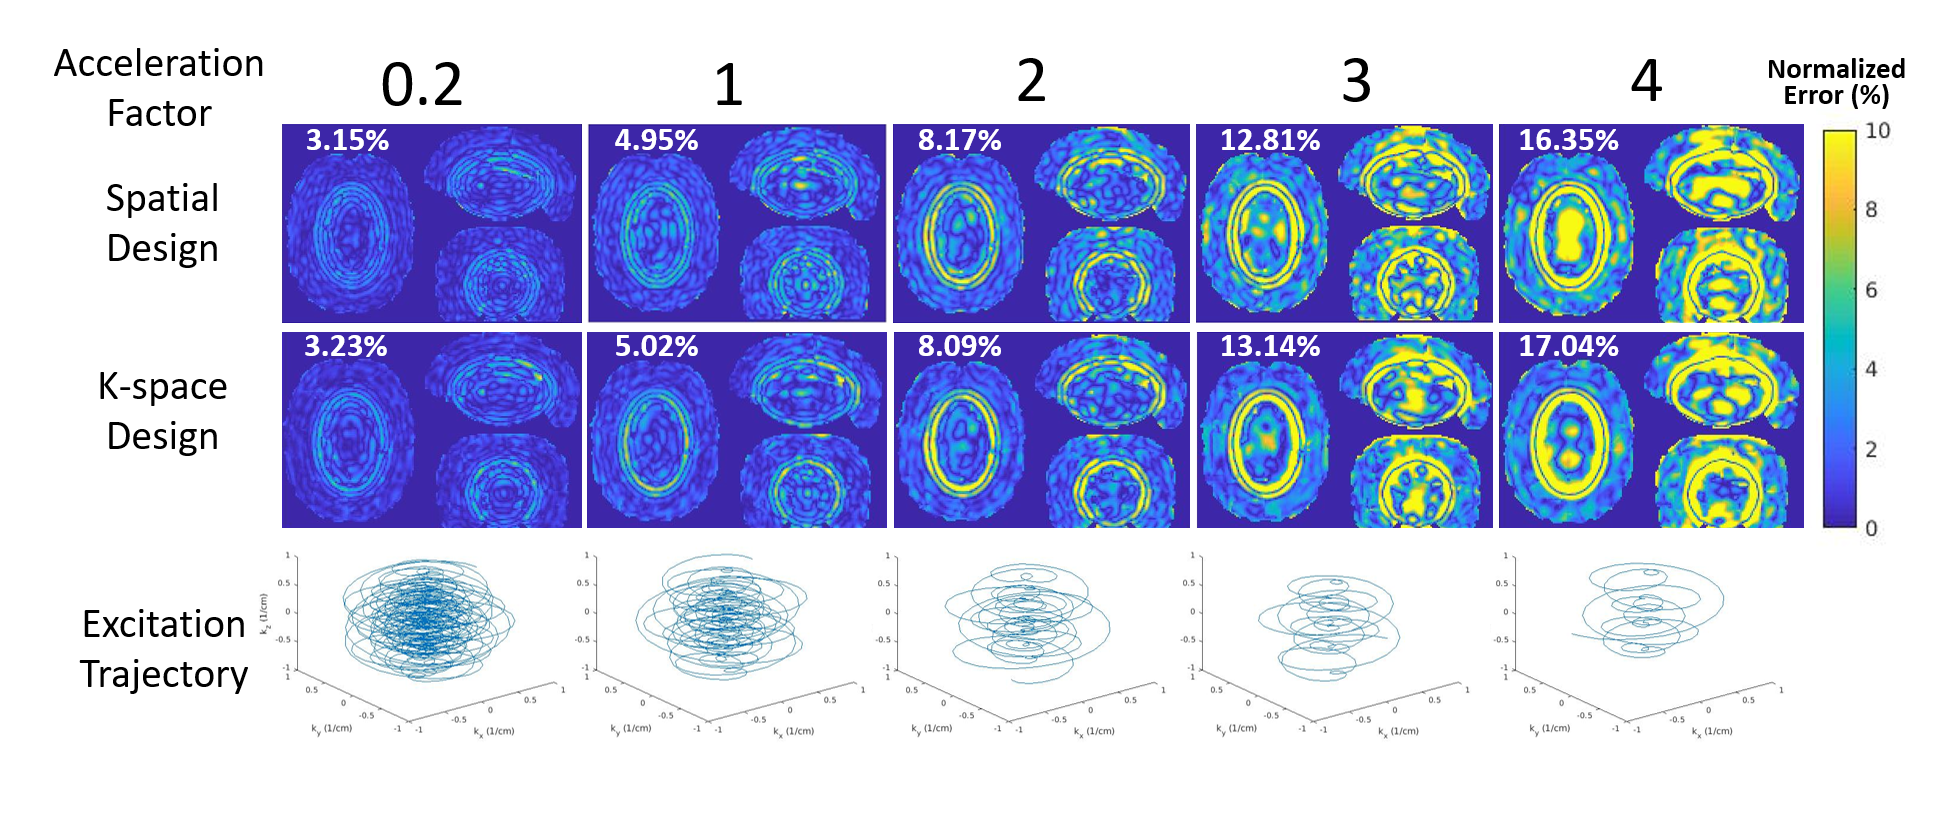
\includegraphics[width=\textwidth]{kspace_PTX_Acceleration}
	\caption{ Normalized error maps and RMSE for spatial domain design (first row) and k-space domain design (second row), with excitation trajectories undersampled by different acceleration factors (third row).}
	\label{fig:kspace_PTX_Acceleration}
\end{figure}

Figure \ref{fig:kspace_PTX_Acceleration} shows a comparison between the performance of spatial domain design (first row) and k-space domain design (second row) regarding undersampled excitation trajectories (third row) with different acceleration factors. Both design methods had larger errors when the excitation k-space was less densely traversed. The k-space domain design provided similar error maps and practically equal NRMSE. The k-space domain design had slightly larger NRMSE because of the interpolation and truncation of the k-space sensitivity when building the $\mathbf{S}^{H}\mathbf{S}$ matrix, and can be improved by increasing the inclusion width. 


\begin{figure}
	\centering
	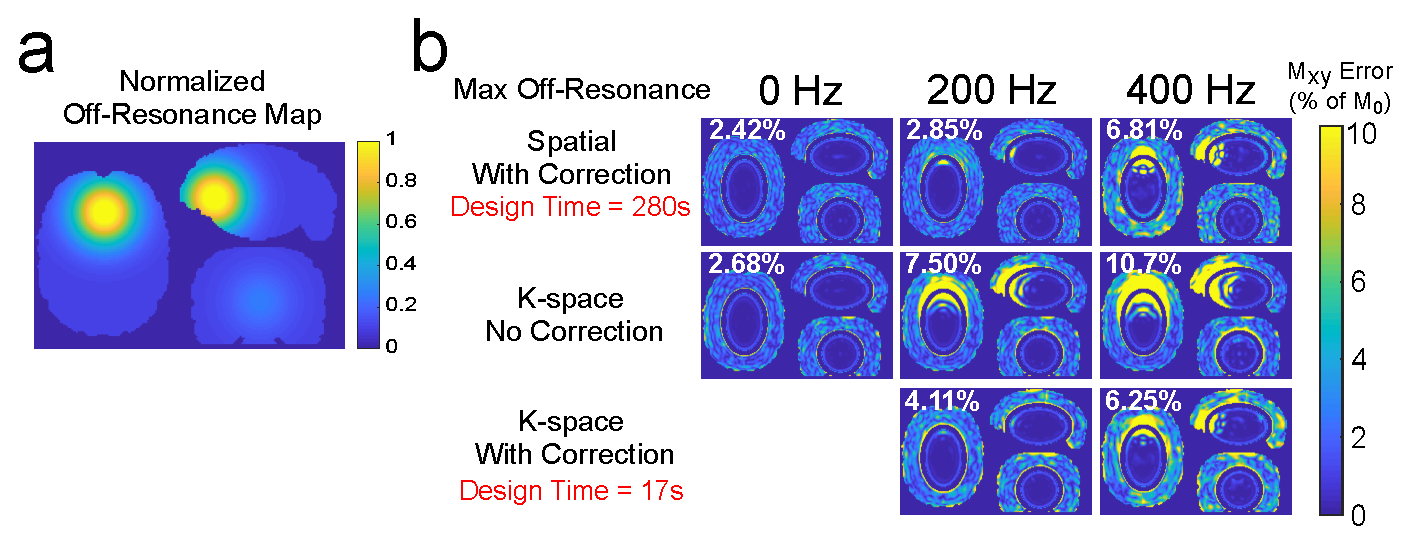
\includegraphics[width=\textwidth]{kspace_PTX_B0}
	\caption{\textbf{(a)} Normalized off-resonance map with Gaussian distortion centered above the frontal sinus, mimicking a characteristic susceptibility induced $B_0$ inhomogeneity. \textbf{(b)} Normalized excitation maps and RMSE for spatial domain design with off-resonance correction (first row), k-space domain design with and without off-resonance correction (second \& third rows).}
	\label{fig:kspace_PTX_B0}
\end{figure}

Regarding 3D off-resonance patterns with the shape shown in Figure \ref{fig:kspace_PTX_B0}a and different scaling, Figure \ref{fig:kspace_PTX_B0}b shows the excitation maps of three types of designs: spatial domain design with off-resonance correction (first row), k-space domain design with and without off-resonance correction (second \& third row). As shown in the second row of Figure \ref{fig:kspace_PTX_B0}b, off-resonance caused false excitation outside the designated suppression region, and must be corrected. k-space domain design with correction was able to correct off-resonance artifacts and provide excitation patterns comparable to spatial domain design, for maximum off-resonance up to 200 Hz, which is the typical range of off-resonance observed in clinical studies. The k-space domain design has a weaker performance with higher off-resonance due to the fact that the time segmentation approximation in Ref \cite{fessler2005toeplitz} was meant to approximate forward models from RF to excitation patterns and does not serve as an accurate approximation to the backward model as we need in the k-space domain design.